\documentclass[journal=nalefd,manuscript=letter]{achemso}
%\setkeys{acs}{articletitle=true}
\usepackage{graphicx}
\usepackage{amsmath}
\usepackage{amssymb}
\usepackage{upgreek}
%\usepackage{subfigure}
\usepackage{xr}
%% This is to use color to hihglight the changes introduced for the revised version
\usepackage{color}
\newcommand{\HI}[1]{\textcolor{blue}{#1}} % use to add anything to the main text.
%%% This is for adding a footer with the time of the compilation of the file.
%%% Useful for versioning of printed copies.
%\usepackage{datetime}
%\usepackage{fancyhdr}
%\fancyfoot[L]{\fontsize{8}{12} \selectfont \today $\,$ \currenttime}
%\pagestyle{fancy}
%%%%%%%%%%%%%%%%%%%%%%%%%%%%%%%%%%%%%%%%%%%%%%%%%%%%%%%%%%%%%%%%%%%%%
%%%%%%%%%%%%%%%%%%%%%%%%%%%%%%%%%%%%%%%%%%%%%%%%%%%%%%%%%%%%%%%%%%%%%

%\usepackage[version=3]{mhchem} % Formula subscripts using \ce{}
\usepackage[T1]{fontenc}       % Use modern font encodings
\externaldocument{supporting}

\newcommand{\K}{\ensuremath{\,\textrm{K}}}
\newcommand{\nm}{\ensuremath{\,\textrm{nm}}}
\newcommand{\mm}{\ensuremath{\,\textrm{mm}}}
\newcommand{\um}{\ensuremath{\,\upmu\textrm{m}}}
\newcommand{\m}{\ensuremath{\,\textrm{m}}}
\newcommand{\eV}{\ensuremath{\,\textrm{eV}}}
\newcommand{\uM}{\ensuremath{\,\upmu\textrm{M}}}
\newcommand{\uW}{\ensuremath{\,\upmu\textrm{W}}}
\newcommand{\mW}{\ensuremath{\,\textrm{mW}}}
\newcommand{\W}{\ensuremath{\,\textrm{W}}}
\newcommand{\pM}{\ensuremath{\,\textrm{pM}}}
\newcommand{\meV}{\ensuremath{\,\textrm{meV}}}
\newcommand{\pwr}{\ensuremath{\,\textrm{kW/cm}^2}}
\newcommand{\fs}{\ensuremath{\,\textrm{fs}}}
\newcommand{\ps}{\ensuremath{\,\textrm{ps}}}
\newcommand{\CPS}{\ensuremath{\,\textrm{CPS}}}
\newcommand{\kCPS}{\ensuremath{\,\textrm{kCPS}}}
\newcommand{\atto}{\ensuremath{\textrm{ATTO}\,647\textrm{N}}}
\newcommand{\degree}{\ensuremath{\,^o\textrm{C}}}

\author{Aquiles Carattino}
\affiliation[Leiden]
{Huygens-Kamerlingh Onnes Lab, 2300RA Leiden, The Netherlands}
\author{Mart\'in Caldarola}
\affiliation[Leiden]
{Huygens-Kamerlingh Onnes Lab, 2300RA Leiden, The Netherlands}
\author{Michel Orrit}
\email{orrit@physics.leidenuniv.nl}
\affiliation[Leiden]
{Huygens-Kamerlingh Onnes Lab, 2300RA Leiden, The Netherlands}

\title{Gold nanoparticles as absolute nano-thermometers}

\keywords{Gold nanorods, Plasmon, Anti-Stokes, Sensing, Temperature}

\begin{document}
%\maketitle

%%%%%%%%%%%%%%%%%%%%%%%%%%%%%%%%%%%%%%%%%%%%%%%%%%%%%%%%%%%%%%%%%%%%%
%% The "tocentry" environment can be used to create an entry for the
%% graphical table of contents. It is given here as some journals
%% require that it is printed as part of the abstract page. It will
%% be automatically moved as appropriate.
%%%%%%%%%%%%%%%%%%%%%%%%%%%%%%%%%%%%%%%%%%%%%%%%%%%%%%%%%%%%%%%%%%%%%
\begin{tocentry}

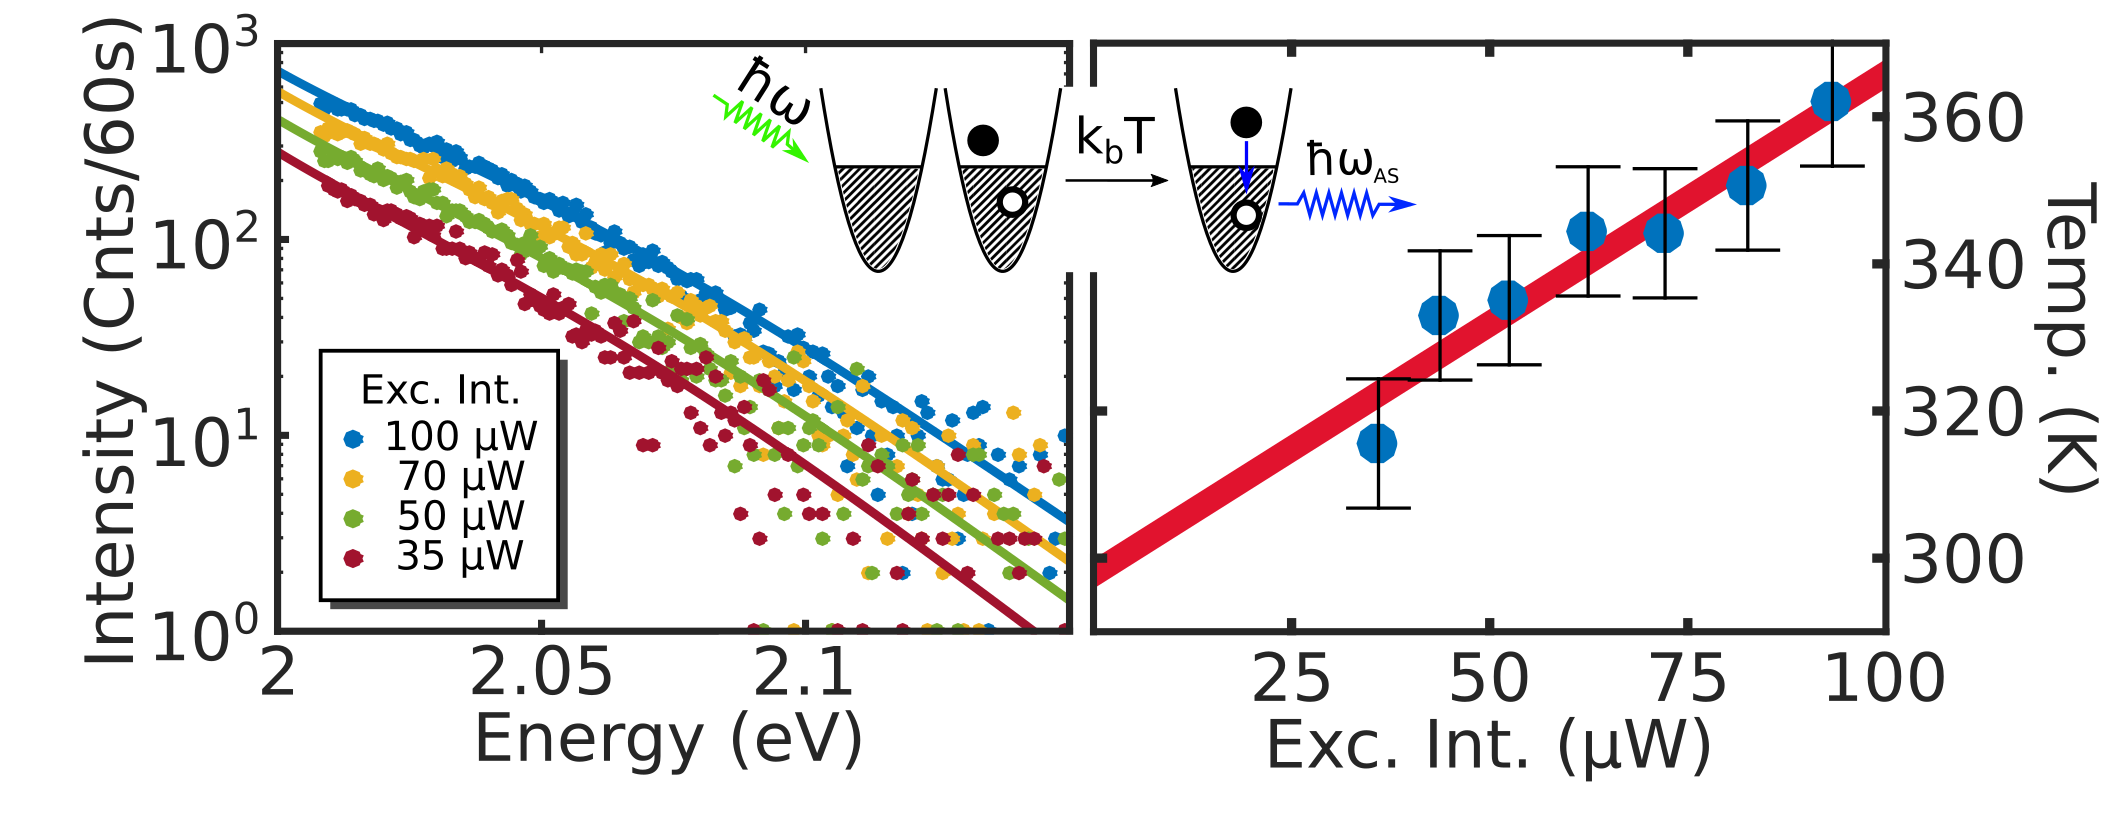
\includegraphics[width=90.0mm]{Figures/00_TOC/TOC.png}

\end{tocentry}

\begin{abstract}
Nano-thermometry is a challenging field that can open the door
to intriguing questions ranging from biology and medicine to material sciences.
Gold nanorods are excellent candidates to act as nanoprobes because they are
reasonably bright emitters upon excitation with a monochromatic source.
Gold nanoparticles are commonly used in photothermal therapy as efficient
transducers of electromagnetic radiation into heat. In this work we \HI{use} 
the spectrum of the anti-Stokes emission from gold nanorods irradiated in
resonance to measure the \textit{absolute temperature} of the nanoparticles \HI{and their
surrounding medium} \textit{without} the need for a previous calibration. 
\HI{We show a $4\K$ accuracy in the determination
of the temperature of the medium with spectral measurements of $180$ s integration time.}
This procedure can be easily implemented in any microscope capable of acquiring emission spectra \HI{and it
is not limited to any specific shape of nanoparticles.} 

\end{abstract}


Most physical, chemical and biological processes depend on
temperature. Together with the miniaturization of devices and the advent of
nanotechnology the need for measuring temperature with high spatial accuracy
started to emerge. Notably in biology\cite{Yang2011a,Hrelescu2010} and
medicine\cite{Li2013c} \HI{measuring and controlling temperature at a sub-cellular 
scale are the challenges that need to be overcome to achieve better understanding and control 
of the mechanisms involved in new therapies such as photothermal tumor ablation\cite{Gobin2007} 
or controlled drug delivery\cite{Huang2006,Huo2014}.}

Nanometer-size probes with distinctive spectral features are ideal candidates
for temperature measurements since they provide high spatial accuracy while
far-field optics allow a non-contact readout. Some of the proposed strategies
include structures that undergo a conformational change upon an increase in
temperature\cite{Ebrahimi2014}, thus inducing variations in fluorescence
intensity of a dye molecule embedded in them.

Also cleverly designed lanthanide-based fluorescent probes in which the ratio of
particular emission peaks depends on temperature \HI{provide} a high accuracy and can
be used as nanothermometers \cite{liu2016ratiometric} even in biological samples
\cite{Vetrone2010}. Photobleaching is often an important limitation of these
approaches. Recently, Surface Enhanced Raman Spectroscopy (SERS) allowed to
measure spectral changes induced by temperature down to single
molecules\cite{Pozzi2015}, but a careful calibration of the measurements is
crucial.

Gold nanoparticles continue to receive a fair amount of attention because of
their unique optical properties\cite{Zijlstra2011}. The collective oscillation
of conduction electrons, also known as plasmon, shows a resonance in the visible to
near infra-red wavelengths. This resonance can be tuned by changing the shape of
the particles\cite{Carattino2016} and is responsible for a large absorption
and scattering cross section at the resonance wavelength. These cross sections can
be calculated by solving the Maxwell equations numerically employing different computer
packages\cite{Draine1994,Yurkin2011,Oskooi2010}, providing a good agreement
between calculations and what is experimentally achievable. 

Thanks to their high absorption and scattering cross section (several times higher
than their geometrical cross section) it is relatively simple to detect
nanoparticles in a dark-field scattering configuration\cite{Hu2008} or via
photothermal imaging\cite{boyer2002photothermal, Berciaud2006}.
Alternatively, detecting gold nanoparticles through their
luminescence\cite{Tcherniak2011} is also possible; their low quantum
yield\cite{Fang2012,Rao2015,Yorulmaz2012,Cheng2015}, \HI{around $10^{-6}$,}	
is compensated by the enhanced cross section at the surface plasmon resonance
(SPR). The luminescence signal is stable over time; gold nanoparticles do not
blink nor bleach, therefore are useful labeling agents for processes that
require extended periods of observation\cite{Wang2005}.

Different metallic nano-objects are being introduced as agents for photothermal
therapy\cite{Huang2006,Huang2008} or drug delivery\cite{Kang2013}. One of the
advantages of gold nanoparticles is the possibility of tuning their resonance to
the near infra-red range, where the penetration of light into tissues can be of
several
centimeters\cite{Huang2006,Gobin2007,Hirsch2003,ONeal2004,Li2013c,Huang2008}.
Moreover the particles can be used not only for treatment, but also for
imaging\cite{Zhao2014a,Huang2006}. In the case of photothermal therapy,
nanoparticles are used as heat sources\cite{Gobin2007,Hirsch2003} to locally
increase the temperature in order to induce the death of specific cells in a
tissue\cite{Huang2008,Huang2006}. However, the temperatures
reached\cite{Donner2013} can only be estimated from models\cite{Zhao2014a} or
from an ad-hoc calibration. Therefore a method to simultaneously increase 
and monitor the local temperature will be of great interest in a
broad range of fields. In this paper we show that the anti-Stokes luminescence
of \HI{single} gold nanorods can be used to measure their temperature 
\HI{upon resonant CW irradiation. The temperature error for a single measurement
is less than $10\K$ with an acquisition time of a few minutes; with a set of such 
measurements, the temperature of the surrounding medium can be determined with 
$4\K$ accuracy or better.}
% Changed the "less than 4K acquiracy", mainly because less is more when talking about accuracy.

Luminescence of metallic nanoparticles has been the subject of extensive study in
recent years. Since the first observation of luminescence from bulk
gold\cite{Mooradian1969}, different groups have tried to quantitatively describe
the observed properties\cite{Mohamed2000,Beversluis2003a} \HI{\cite{Huang2014, hugall2015demonstrating,mertens2017light}}, 
such as the quantum yield\cite{Fang2012,Rao2015,Yorulmaz2012,Cheng2015,Dulkeith2004} and the
emission spectrum\cite{Link2010}. In particular, gold nanorods present two distinct
resonance energies, namely the transverse and the longitudinal plasmon
resonances. These particles can therefore be excited efficiently at one of those
energies; the transverse resonance corresponds to a wavelength of about $530\nm$ and will give
rise to a broad luminescence emission with a peak at the longitudinal plasmon energy.
Conversely it is possible to excite the particles with a wavelength matching
the longitudinal plasmon resonance. In this case the excitation benefits from
an enhanced absorption cross section, but the emission that overlaps the plasmon
resonance will be mostly blocked by the filters needed to prevent direct
excitation light from reaching the detectors.

\HI{In this work, we call ``photoluminescence'' any secondary light  emission \cite{Orrit-Kottis} at energies
different from the excitation laser energy, $\hbar \omega_\textrm{L}$. After (virtual or real)
\footnote{we do not specify whether the absorption is real or virtual.} absorption 
of an excitation photon, the excited electronic state \cite{Mooradian1969,Dulkeith2004} 
may interact and exchange energy with the
phonon bath or, in the case of metals, with the bath of thermally excited charge carriers around the
Fermi level. After a number of interactions, the excited electronic state will re-emit a 
photon which can possess a lower or higher energy than that of the excitation photon
\cite{Hodak2000,Giri2015,Arbouet2003a}. For a non-resonant excitation, the probability 
of more than one interaction is negligible and the main contribution to secondary emission 
is Raman scattering \cite{Huang2014}. This is the case, for example, of insulators excited 
well below their electronic absorption edge. For resonant excitation, a relatively long-lived 
excited state is prepared. It will have enough time to interact repeatedly with thermal baths, 
particularly with phonons. This is the case of organic dye molecules or
semiconductors, in which relaxed fluorescence is observed. We also note that fluorescence 
always presents hot bands on the anti-Stokes side of the excitation laser. In most 
fluorescence detection schemes, however, these hot bands are ignored, but they are 
far from negligible in heavily doped samples\cite{Carattino2016a}.}

\HI{Metal nanoparticles fall between those two extremes because the excited electronic state, 
an electron-hole pair, relaxes very rapidly by interacting with other charge carriers and with phonons. 
The photoluminescence lifetimes are on the order of tens of femtoseconds\cite{link1999} and 
therefore there is not enough time to obtain a fully relaxed luminescence. In other words, the 
photoluminescence is always ``hot''. It is worth noting that Raman scattering, 
corresponding to the lowest order of interaction with baths, will be an important
contribution to photoluminescence\cite{Huang2014,mertens2017light}. However, second 
and higher orders may also contribute significantly. Because all these processes obey a 
Boltzman-type of relation between anti-Stokes and Stokes emission, they cannot be easily 
distinguished from each other on the basis of their temperature dependence.}


\HI{The anti-Stokes emission is highly sensitive to temperature and thus 
it can be used for thermometry\cite{xie2016thermometry}. In this letter we present 
a simple procedure to extract the absolute temperature from the anti-Stokes 
photoluminescence spectrum of individual gold nanorods without the need of 
any previous temperature calibration. We show that we can determine the particle temperature 
\textit{in-situ} with an accuracy of $6\%$ by recording a single anti-Stokes spectrum (with an 
acquisition time of $3$ minutes). 
Moreover, by performing this measurement at different excitation powers 
we can obtain the temperature of the surrounding medium with an accuracy better than $2\%$.}

\HI{\textbf{Phenomenological model for the luminescence emission.} 
In a nutshell, we consider the luminescence emission as radiative recombination of
electron-hole pairs created by the decay of the plasmon and safter their interaction
with thermal baths. Before the recombination, carriers may interact with the baths one or more
times, leading to secondary light emission with an energy different from the initial internal energy of the pair. 
The anti-Stokes spectral contribution arises from interactions that increase the energy 
of the pair, whereas the Stokes emission to a decrease in energy. The emission process will be 
enhanced by the plasmon; therefore the luminescence spectrum will be modulated with the plasmon shape. 
A scheme of these ideas is shown in the Supporting Information.}

\HI{Exciting a gold nanorod with a monochromatic beam at its resonance frequency, $\omega_\textrm{SPR}$, generates a collective oscillation of the gas of conduction electrons, also called a plasmon.} 
%The lifetime of this oscillation can be measured in
%pulsed experiments or estimated from the inverse of the linewidth and is in the
%order of $10\fs$\cite{link1999,Sonnichsen2002} (neglecting any dephasing time $T_2^*$).
The plasmon decays by forming a pair of hot electron and hole with an internal energy equal to the exciting
photon energy\cite{Sundararaman2014,Brongersma2015,AlejandroManjavacasJunG.LiuVikramKulkarni2014}, 
i.e. \HI{ $E_{e-h}=\hbar \omega_\textrm{L}$.}

%The hot electron and hole cool down by exchanging energy with the lattice on a
%timescale of $\tau\approx1\ps$\cite{Pustovalov2005}. 
This hot electron and hole have a small probability of recombining radiatively, i.e. of 
re-emitting their high electronic energy as a photoluminescence photon. If they
have interacted only with static surfaces or defects, their energy will be the same and
therefore the emitted photon will have the same energy as the incoming
photon, and will not contribute to the measured photoluminescence. It will be
blocked by the notch filter used to remove the exciting laser from detection.
If, on the other hand, they have interacted with a
phonon or a thermally excited electron or hole, they may have lost or acquired
energy.
% by creation or annihilation of phonons or interact with thermally excited charge carriers. 
In both cases the energy available upon
recombination cannot much exceed $\hbar\omega_L+k_\textrm{B}T$, \HI{where $k_\textrm{B}$ 
represents Boltzmann's constant and $T$ the absolute temperature.} 
%It has to be noted that in the hypothesis of a single-photon absorption at low 
%excitation power, the temperature $T$ is that of the baths before absorption, i.e. the temperature of
%the medium surrounding the particle. This is different from pulsed experiments,
%in which the electron gas temperature can be orders thousands of K higher than
%room temperature\cite{Baffou2013a}. 

Radiative recombination gives rise to emission spectrally and
spatially distributed throughout the particle over a broad frequency band with
an exponential cutoff at $\hbar\omega_\textrm{L}+k_\textrm{B}T$. The weak
recombination emission can be greatly enhanced by the surface plasmon resonance,
acting as an antenna. 
%Supplementary figure S1 shows a schematic representation of the described processes. 
With this model the following predictions can be made.
Firstly the emission spectrum must follow the plasmon spectrum if the excitation
laser is well above the plasmon resonance as shown in \mbox{Figure
\ref{fig:spectra_intensity}}, \HI{green line}. If the excitation falls within the
plasmon resonance, the spectrum is expected to follow the plasmon spectrum
multiplied by a Bose-Einstein statistics factor arising from phonon population. 
\HI{Here we assume that the coupling to the phonons dominates the process, while references
\cite{Huang2014,mertens2017light} assume that carrier-carrier interactions dominate.
Thus, under our assumption, the emission} should be proportional to the \HI{phonon occupation} number $\bar{n}$ 
for anti-Stokes and $\bar{n}+1$ for Stokes processes, with

\begin{equation}\label{eqn:BE}
	\bar{n}=\left(\exp\frac{\hbar\Omega}{k_\textrm{B}T}-1\right)^{-1}\,,
\end{equation}
\HI{where $\hbar\Omega$ is the phonon energy. It is possible to consider 
carrier-carrier interactions obeying Fermi statistics, i.e. $n=\left(\exp(\frac{\hbar \Omega}{k_\textrm{B}T})+1 \right)^{-1}$\cite{Huang2014,mertens2017light}.} 

With this model, we can also predict that the emission should be polarized. 
For the strong longitudinal plasmon of gold nanorods this polarization coincides with
the longitudinal axis of the particle\cite{He2015}. Moreover, the lifetime
should be determined by the lifetime of hot electrons and holes and should be
significantly shorter than the thermalization time of the carriers. 
Indeed, a few interactions would suffice to reduce the carriers' energy significantly
and therefore the electron and hole wouldn't have the energy required to produce an
optical photon. 
%Finally, only the presence of hot carriers is required in the model. 
One important assumption for this model is that the emission spectrum
of radiative recombiantion is much broader than the plasmon. 
Therefore excitation \HI{just} above the plasmon resonance should excite the 
electron-hole pairs with nearly the same efficiency as well above the plasmon
resonance\cite{Cheng2015,mertens2017light}. 

\HI{\textbf{Application to nanothermometry.} According to the model just
described, the anti-Stokes emission spectrum follows the form,}

\begin{equation}\label{eqn:fitting}
	I(\omega) =
	\textrm{I}_{\textrm{SPR}}(\omega)\cdot\left(\exp\frac{\hbar(\omega-\omega_\textrm{L})}{k_\textrm{B}T}-1\right)^{-1}
\end{equation}

\noindent where $I(\omega) $ is the emitted intensity, $\omega$ is the angular frequency
of the photons and $\omega_\textrm{L}$ is the frequency of the \HI{exciting} laser.
%, $\hbar$ is Planck's constant, $k_\textrm{B}$ Boltzmann's constant.
$\textrm{I}_{\textrm{SPR}}(\omega) $ is the surface plasmon resonance \HI{profile} that 
will be obtain by exciting the particle at energy much higher than the resonance. The
only remaining free parameter is the temperature $T$ (and a normalization
constant not included in equation \ref{eqn:fitting}). \HI{Fitting  
measured anti-Stokes emission spectra with this equation will 
yield the absolute temperature $T$ of the particle under study.}

\HI{The procedure we propose to obtain the absolute temperature of gold nanorods 
form the anti-Stokes luminescence emission and without 
the need of any previous temperature calibration involves the following steps.}

\HI{
\begin{enumerate}
	\item Obtain the plasmon resonance spectrum of the particle. This is usually expressed as a 
	Lorentzian function \cite{Zijlstra2011}, i.e.
	\begin{align*}
	\textrm{I}_{\textrm{SPR}}(\omega) &= \frac{\left( \Gamma/2 \right)^2}{\left( \omega-\omega_\textrm{SPR}\right)^2 +
	\left( \Gamma/2 \right)^2} 
	\end{align*}
	where $\omega$ is the photon energy frequency, $\omega_\textrm{SPR}$ is the resonance frequency 
	and $\Gamma$ is the width of the surface plasmon resonance.
	In our case, we detect the spectrum of photoluminescence,	excited at $532\nm$ to extract 
	$\omega_\textrm{SPR}$ and $\Gamma$, as explained in the Supporting Information, along with an explanation of the 
	experimental errors. 
	\item Excite near the longitudinal plasmonic resonance and detect the blue-shifted anti-Stokes emission spectra. For this we employed a $633\,$ nm  laser as a source. 
	\item Fit the high-energy part of the spectrum using equation \ref{eqn:fitting} with $T$ as the \textit{only} free parameter.
\end{enumerate}
}

\HI{We emphasize that we cannot simply use the anti-Stokes to Stokes intensity ratio to 
obtain the temperature of the particle, as is commonly done with Raman lines of molecules 
\cite{krishnan1928influence,zondervan2006single}, due to the presence of the strong plasmonic enhancement
of the emission that must be considered in addition to the Boltzmann factor.}

\HI{\textbf{Experimental method.}} All the measurements in this work were performed with a home-built confocal
microscope equipped a spectrometer (Acton 500i) in the emission path.  We focused
our lasers to a diffraction-limited spot using a $60\times$, NA $1.4$ oil immersion
objective (Olympus) and collected the emitted photons through the same
objective. This provided high excitation and collection efficiency.
We employed a $532\nm$ (CNI) laser for characterizing the nanorods' plasmon and
a $633\nm$ HeNe (Thorlabs) to excite the nanorods in resonance.
We give more experimental details in the Supporting Information.

Wet chemically synthesized nanorods\cite{Nikoobakht2003} with average dimensions
of $21\nm\times50\nm$ and a plasmon resonance around $650\nm$ were spin-coated
onto clean coverslips, controlling the superficial concentration to separate
individual nanorods within the diffraction-limited spot\cite{Zijlstra2011}.
In addition, the samples were mounted in a flow cell that allowed us to increase
the temperature of the medium up to $60\degree$ and to monitor it through a
Pt100 resistance thermometer placed $1\mm$ away from the observation area. More
details about the experimental setup are given in the Supporting Information.

To compensate for the drift of the setup while increasing the temperature, we
developed a computer program to continuously track a reference particle. The
same program was responsible for recording the temperature and triggering the
spectrometer. In this way complete data sets were acquired at different
temperatures, with excitation at $532\nm$ and $633\nm$, at
different laser intensities. A
spectrum with $532\nm$ laser excitation was taken after every cycle to ensure
that the particle under study had not reshaped due to high excitation power.

The intensity of the laser was controlled via an acousto-optic modulator. 
\HI{Six accumulations of each spectrum were recorded with an exposure 
time of $30$ s.} This not only allowed us to
lower the noise of the measurement because of a longer exposure time 
(\HI{$3$ minutes in total}), but also allowed us to remove bright pixels generated by cosmic rays. 
Having several accumulations is also useful to monitor changes in the intensity of the spectra
during the acquisition itself. These changes can be due to a drift of the setup
while measuring or to a reshaping of the particle. If the reshaping was
confirmed by comparing the spectra acquired with the $532\nm$
laser\cite{Liu2009}, the measurements where rejected. If the changes in the
observed emission spectra were due to drift of the setup, the particular data
set was not taken into account. For the purposes of this work the excitation
intensity is crucial for characterizing the method; if the particle is not in
focus it would result in an overestimation of the excitation power. 

% \section{Results}


\HI{\textbf{Experimental Results.}} The proposed model for the anti-Stokes emission requires the plasmon
spectrum ($\textrm{I}_{\textrm{SPR}}(\omega)$ in equation \ref{eqn:fitting}) 
in order to fit the emission at shorter wavelengths and extract the
particle temperature. It has been shown that both scattering and luminescence
spectra roughly overlap over a broad range of wavelengths\cite{Yorulmaz2012}. Therefore
exciting gold nanorods with $532\nm$ allows us to record the longitudinal
plasmon spectra, as shown in the green solid curve of Figure \ref{fig:spectra_intensity}. 
\HI{It has to be recalled that the luminescence spectrum is not a perfect
Lorentzian since there is a broadband contribution also observed in bulk gold \cite{Mooradian1969}.
The procedure to extract the SPR profile from such a measurement is explained in the
Supporting Information. We show in figure \ref{fig:spectra_intensity} the extracted 
surface plasmon profile in the red solid curve. }
%was fitted by a single Lorentzian, shown in red in the Figure; the dashed
%part of the curve is the spectral region that was not considered for the
%fitting. 
%to the luminescence arisingbetween the excitation wavelength and the plasmon peak\cite{Boyd1986}. 
%This appears as an asymmetry in the emission spectrum, particularly visible for
%wavelengths smaller than $625\nm$. The results of this fitting will be employed
%for the $\textrm{I}_\textrm{SPR}$ function defined in equation \ref{eqn:fitting}. 

\begin{figure}[tp] \centering
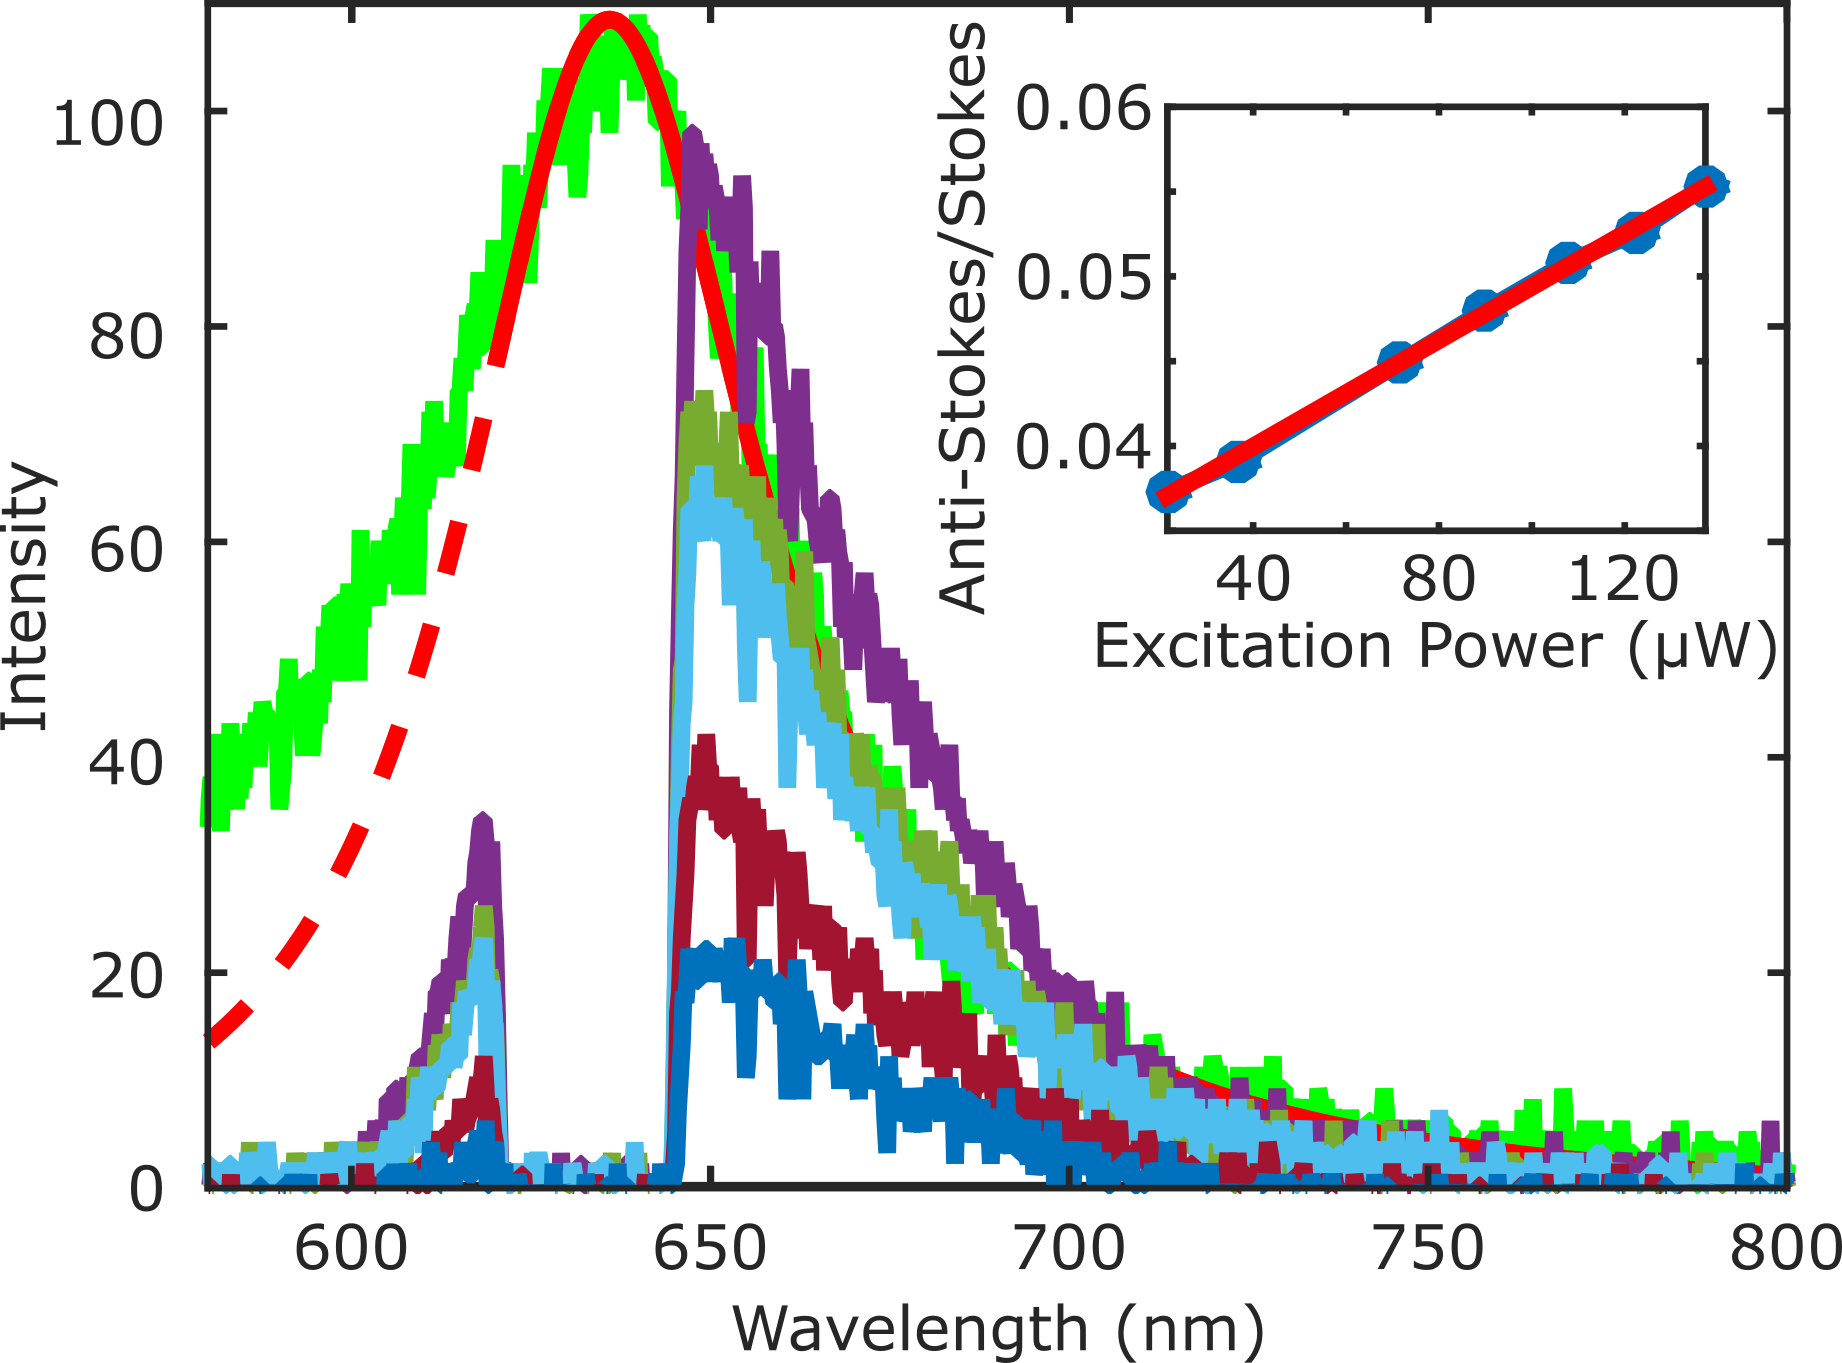
\includegraphics[width=78.4mm]{Figures/02_Several_Intensities/02_several_intensities.png}
\caption{\textbf{Luminescence emission spectra of a single gold nanorod.} The green curve is the
measured luminescence emission under $532\nm$ excitation \HI{and the red curve shows the 
extracted $\textrm{I}_{\textrm{SPR}}(\omega)$ from this spectra.}
The other curves are the emission of the same particle under $633\nm$ irradiation at three 
different powers indicated in the legend. The inset shows the anti-Stokes-to-Stokes ratio as a function
of the excitation power, overlapped with a linear fit in red. The dip centered on the laser wavelength
is caused by the notch filter used to prevent the excitation laser from reaching the detectors.}
	\label{fig:spectra_intensity}
\end{figure}

The other curves in Figure \ref{fig:spectra_intensity} show the luminescence emission of
the same nanorod with irradiation at $633\nm$ at different powers,
ranging from $25\uW$ to $75\uW$ at the back aperture of the objective.  
%% should change to intensity or clearly mention the spot size
The vertical black line shows the wavelength of the laser. The Stokes part of the
spectrum at longer wavelengths than the excitation shows the same shape as the
plasmon emission observed under $532\nm$ excitation, apart from a normalization
factor. From the figure it can readily be seen that the shape of the anti-Stokes
emission, at shorter wavelengths than excitation, is exponential-like and
doesn't follow the Lorentzian shape of the Stokes emission. The dip between
Stokes and anti-Stokes is caused by the notch filter that prevents direct
excitation light from reaching the detectors. 

The inset of Figure \ref{fig:spectra_intensity} shows the anti-Stokes-to-Stokes ratio of
the integrated luminescence for different laser excitation intensities. It is
possible to see that even though the photoluminescence process is linear with a 
linear behavior, the anti-Stokes intensity increases slightly more rapidly than the Stokes emission.
We already exploited this phenomenon to image gold nanorods in high-background
conditions\cite{Carattino2016a}. 
%The anti-Stokes emission
%depends on laser excitation power slightly differently from its Stokes counterpart. 
For more information on the power dependence of both the anti-Stokes and Stokes luminescence, 
please refer to the Supporting Information. 

\begin{figure}[tp] \centering
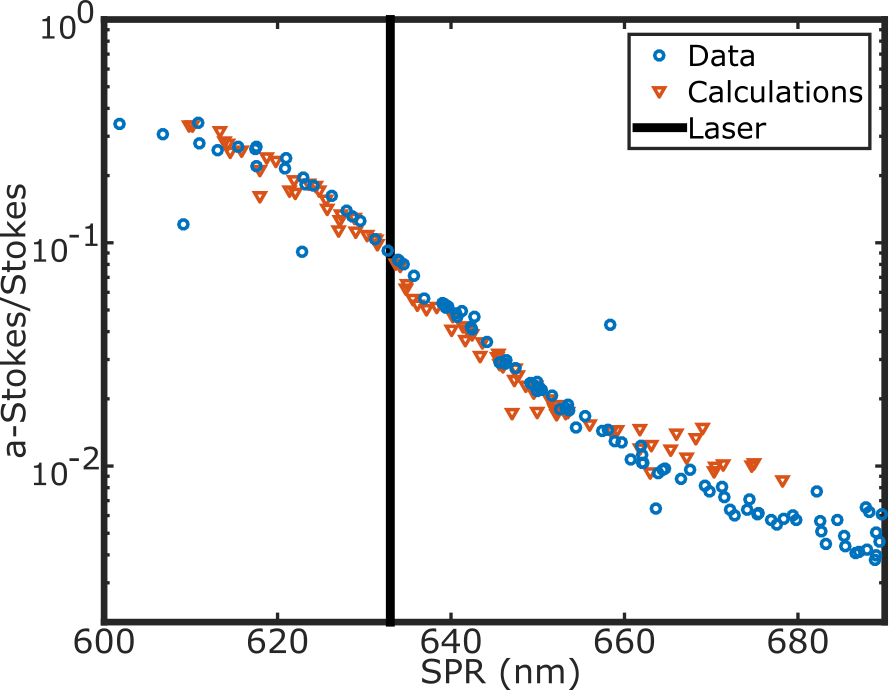
\includegraphics[width=75.5mm]{Figures/02_AS_vs_S_SPR/02_AS_vs_S_SPR.png}
\caption{\textbf{Characterization of anti-Stokes emission for different surface plasmon resonance.} 
Ratio of the anti-Stokes to Stokes emission under $633\nm$ excitation
as a function of the resonance wavelength of the particle.
The blue circles are experimental results (\HI{$105$ different nanorods}), while the red triangles are the
results of numerical simulations with equation \ref{eqn:BE} (\HI{$82$ nanorods with different aspect ratio}). 
There is a very good agreement between experiment and calculations. Particles with a resonance
to the blue of the laser (indicated by the vertical red line) have an increased anti-Stokes
emission.}
	\label{fig:ASS-ratio}
\end{figure}

To further characterize the anti-Stokes emission in gold nanorods, we measured the emission for \HI{$105$}
nanorods with different plasmon resonances under the same $633\nm$ excitation
and calculated the ratio of integrated anti-Stokes to Stokes emissions.
Figure \ref{fig:ASS-ratio} shows the experimental ratios as blue circles, where
as a function of the surface plasmon resonance (SPR) of the
particle. The vertical red line marks the laser wavelength. The particles measured 
had resonances between $600\nm$ and $690\nm$; the ones showing the
maximum ratio of anti-Stokes to Stokes are those with a resonance to the blue of
the laser. For these particles the longitudinal plasmon is enhancing preferably the
anti-Stokes emission. For particles with a resonance at the laser wavelength the
anti-Stokes and the Stokes emission have similar enhancement and show a ratio
close to $10\%$.

Figure \ref{fig:ASS-ratio} also shows as red triangles the results of numerical calculations following
the protocol presented before. 
An excellent overlap between the measured and the calculated data can
be observed. The absorption cross section of \HI{$82$} particles was calculated numerically
with the ADDA package\cite{Yurkin2011} \HI{using a fixed width of $23\nm$ and different 
lengths to achieve different SPR wavelengths. In the Supporting Material we 
show TEM images from which we extracted the size of the nanorods.}
Each calculated absorption spectrum was 
fitted by a Lorentzian and used as $\textrm{I}_{\textrm{SPR}}(\omega)$ in eqn.
\ref{eqn:fitting}. Assuming a diffraction-limited laser spot and using the
calculated absorption cross section we calculated the temperature of
the particle. This value was used in equation \ref{eqn:fitting} to compute the
anti-Stokes emission spectrum. The Stokes emission was set proportional to the
excitation power  with a shape given by the calculated absorption spectra. Since both
anti-Stokes and Stokes emissions are proportional to the excitation power, this
term cancels out when computing the ratio. The laser power therefore only enters
into the equation when calculating the temperature of the particles. It is
remarkable that the agreement between data and calculations was achieved
without free parameters, solely taking into account the transmission spectra of
the filters.

\begin{figure}[tp] \centering
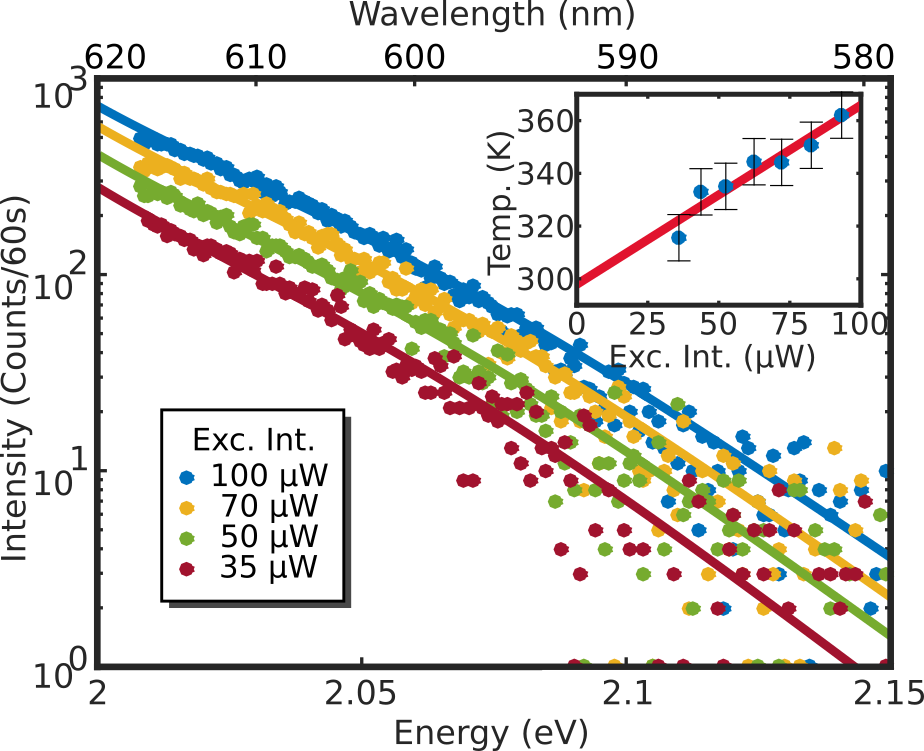
\includegraphics[width=78.4mm]{Figures/03_Fit_Of_AS/03_Log_Fit_AS.png}
\caption{\textbf{Anti-Stokes emission of a single nanorod at different irradiation powers.} We used 
the model from equation \ref{eqn:fitting} to fit the experimental data. 
There is an excellent agreement between data and model. The inset shows the extracted
temperature at each power (blue dots) and a linear 
extrapolation of the data to $0\uW$ excitation power.
The value obtained for room temperature was $293\K$ while the measured value was
$296\K$.}
	\label{fig:AS_in_Log}
\end{figure}

Furthermore, by fitting the anti-Stokes part of the spectra shown in Figure
\ref{fig:spectra_intensity} with equation \ref{eqn:fitting} it is possible to extract
the temperature of the particle at each excitation power. Figure
\ref{fig:AS_in_Log} shows the results of this procedure. The spectra shown were
recorded at $4$ different excitation intensities while the full lines are the
fits; again, there is an excellent agreement between data and model. For every
anti-Stokes measurement we have also acquired the full plasmon spectrum 
exciting with a $532\nm$ laser before and after the temperature extraction.
The full plasmon spectrum is necessary to calculate the parameters of
$\textrm{I}_\textrm{SPR}(\omega)$ from equation \ref{eqn:fitting} and also to verify that the
particle did not reshape while being excited at resonance. 

The inset in Figure \ref{fig:AS_in_Log} shows the temperatures resulting from
the fits at different irradiation intensities (blue dots). Note
that the absolute temperatures of the particle at each excitation power were
calculated without any calibration. As expected, the temperature of the nanorod
\HI{varied linearly with} excitation intensity, or equivalently with the absorbed
energy. Thus, this method provides an \textit{in situ} way to measure the
temperature reached by nanoparticles when they are excited with resonant
monochromatic light. Additionally, from these data sets it  is also possible to
calculate the temperature at $0\uW$ excitation power, i.e. room temperature, by
extrapolating the results with a linear fit. The value we obtained in this case
is $293\pm 6 \K$, while room temperature was $296\K$, a $2\%$ accuracy.

\HI{The accuracy of the obtained temperature depends on an accurate
modeling of the photoluminescence. The first step in the \HI{protocol} is the determination
of the surface plasmon spectral profile, $\textrm{I}_\textrm{SPR}(\omega)$ in equation \ref{eqn:fitting}. 
In this paper we obtained this term by fitting an exponential background plus a Lorentzian to the spectra
obtained at $532\nm$ excitation, as explained in detail in the Supporting Information. We note
that this choice was made for experimental convenience in our setup, but other options to
obtain the SPR profile, are suited for the procedure as well.}
%fitting a Lorentzian to the emission spectrum obtained while irradiating with a
%$532\nm$ laser. In figure \ref{fig:spectra_intensity} it is possible to observe
%that the emission spectrum is not perfectly Lorentzian and therefore the fitting
%results will be sensitive to the portion of the spectrum selected. Depending on
%the wavelength range selected, the parameters of the Lorentzian fit (its width
%and peak position) can slightly change therefore giving rise to different
%temperatures when fitting the anti-Stokes emission spectrum. \HI{For a more detailed 
%discussion of the errors in the temperature determination, see the Supporting Information.} 
%Equation \ref{eqn:fitting} shows that when the resonance is to the red
%of the laser, the term $\textrm{I}_\textrm{SPR}(\omega)$ will vary slowly in the region where the
%anti-Stokes emission is observed. Therefore small errors in the parameters of
%the Lorentzian fit will have a small effect on the temperature extracted.
%However, particles that are not in resonance with the excitation laser will
%present a lower emission due to a smaller absorption cross section and to a
%lower enhancement of the anti-Stokes emission (see for example figure
%\ref{fig:ASS-ratio}). 
%A balance between the amount of collected light and the
%uncertainty produced by the correct determination of the plasmon resonance has
%to be reached depending on each application.
\HI{The error bar in the inset of figure \ref{fig:AS_in_Log} and in the following figures 
is the result of the estimated variance in the fit parameters for the 
anti-Stokes spectra using equation \ref{eq:fitting}, step 3. in our protocol.}

%\HI{We should mention that there are different strategies that can lead to 
%a reduction of the error. For example, longer exposure times for spectra acquisition 
%should yield a better signal to noise ratio, andthe limiting factor of the 
%method is the quality of the $I_\textrm{SPR}(\omega)$ function. It is possible to 
%measure $I_\textrm{SPR}(\omega)$ employing a different technique, such as dark-field 
%spectroscopy, which gives access to the scattering plasmonic resonance. In this case, 
%the better fitting of the plasmonic resonance with a Lorentzian allows one to neglect 
%the shift between absorption and scattering spectra. 
%The exponential-like shape of the anti-Stokes emission implies that a great portion 
%of the emitted light is blocked by the noth filter. Narrower filters will give rise 
%to a substantial increase in signal and perhaps it will open the posibility to test 
%whether Fermi or Bose statistics should be used.}

As expected from the model, the anti-Stokes emission depends not only on
the particle's intrinsic properties but also on the temperature of the
surrounding medium\cite{Konrad2013}. In order to \HI{further} test this point, we changed the
temperature of the sample in a controlled manner and recorded the luminescence
emitted by a single nanorod.

For this set of experiments we employed an air objective ($60\times$, NA $0.9$,
Olympus) to avoid the presence of a heat sink directly in contact with the
observed area. We employed higher laser powers to compensate for the lower
excitation efficiency. At each temperature, \HI{$7$} spectra were acquired at different
$633\nm$ excitation powers and also a spectrum of the plasmon before and after
each measurement in order to monitor any possible reshaping of the particles
during the experiment.

\begin{figure}[tp] \centering
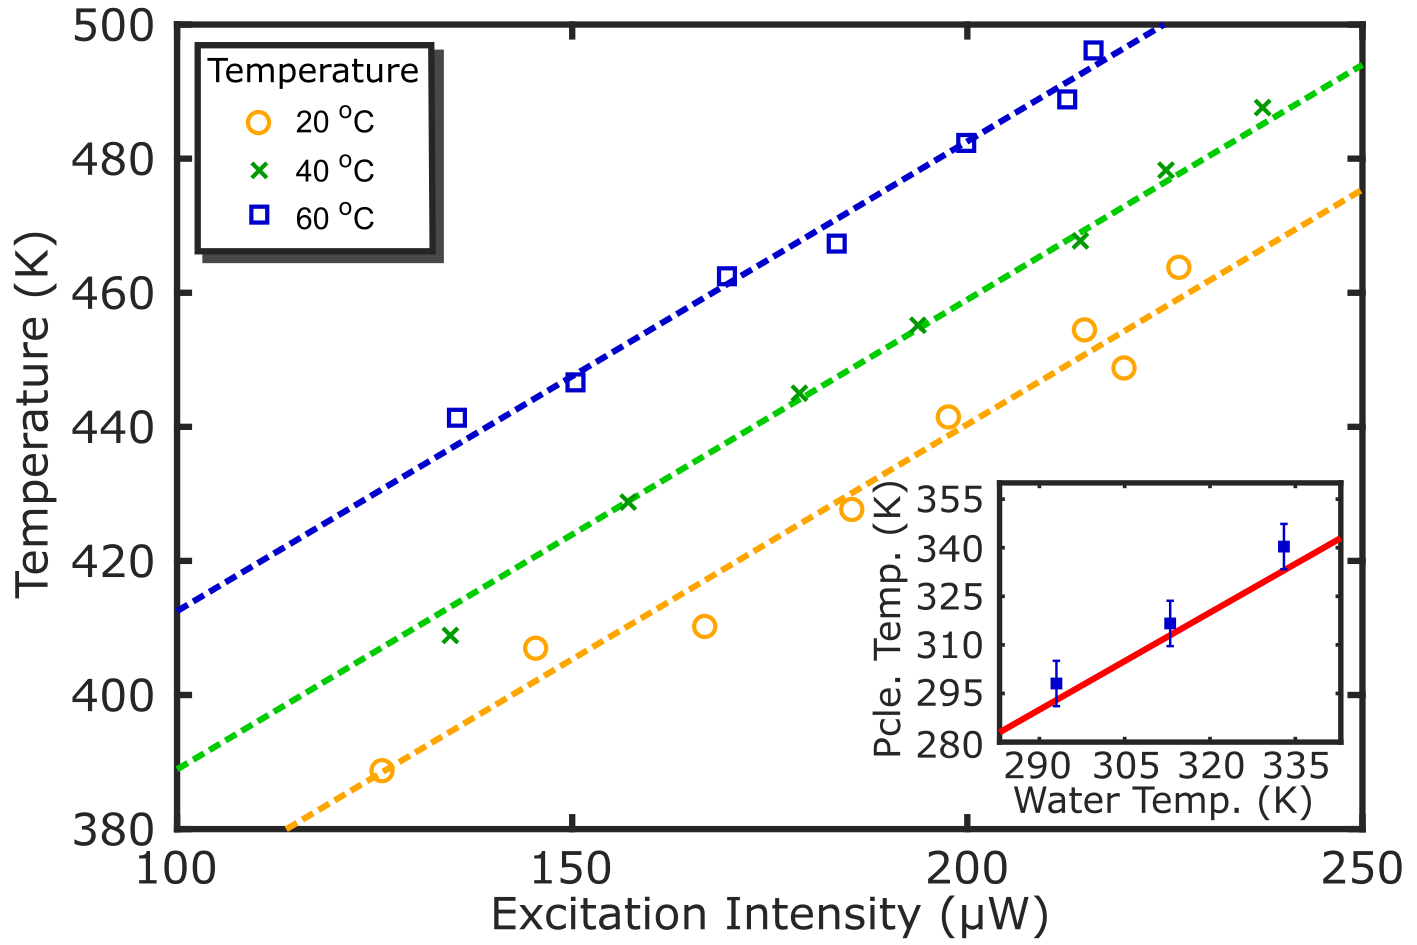
\includegraphics[width=88.4mm]{Figures/03_Fit_Of_AS/03_Log_Fit_AS_02.png}
\caption{\textbf{Calibration-free temperature measurement.}
Extracted temperatures from the anti-Stokes-luminescence emission of an individual nanorod
at different excitation powers and at different sample temperatures. 
The dashed lines lines are fits with the same slope for the three temperatures. 
The \HI{squares} in the inset plot show the local temperature of the sample obtained
by extrapolating \HI{the} temperature at zero excitation power as a function of the water temperature.
The red line represents the expected curve if both temperatures are identical (equal). The dashed blue
line is a fit to the data points with unit slope that shows a systematic offset of $3.8\K$, a $1.2\%$ difference.}
	\label{fig:AS_temp}
\end{figure}

% this paragraph is not so clear to me since it looks there is a loop on the
% room temp determination

Figure \ref{fig:AS_temp} shows the extracted temperature of a particle at
varying excitation powers and at different water temperatures. The blue squares
are the results of the measurement at $20\degree$, while the green crosses are measured
at $40\degree$ and the yellow circles at $60\degree$. The full lines are the
calculated temperatures for a particle with plasmon overlapping the measured one
and assuming a diffraction-limited focus spot. For the dimensions of the
particle, the mean values from TEM images were used and the length was adjusted
to obtain the measured resonance. There is a remarkable agreement between the
calculation and the measured values. Moreover it is possible to extrapolate the
temperature at zero excitation power for each case as was explained earlier. The
results are shown in the inset of the figure for each temperature. The red line
with slope $1$ is a guide to the eye.

Figure \ref{fig:AS_temp} clearly shows that the extracted temperature varies
with the temperature of the surrounding medium. More strikingly the method does
not require any previous calibration nor adjustment. The values obtained with
the extrapolation to $0\uW$ excitation power were $296 \pm 4\K$, $315\pm 4\K$
and $339 \pm 4\K$ for water temperatures of $293\K$, $313\K$ and $333\K$
respectively. The inset plot in figure \ref{fig:AS_temp} presents these points 
and a red solid line with the expected curve if both temperatures are identical. The 
dashed line shows a fit of the data that evidences a small systematic offset of $3.8\,\K$. This represents
an inaccuracy of $1.2\%$ which is a good result for a calibration-free method.
Notably, the presented calibration-free procedure would allow us to perform the same
measurements in any other setup and could act as a reference for calibration of
other nano-thermometers.

%\section{Conclusions}

Being able to control and monitor temperature at the nanoscale is of utmost
importance in different fields ranging from photothermal therapy\cite{Huang2006}
to nano fabrication\cite{Fedoruk2013}. In this work we have shown a simple
procedure that allows us to measure the temperature of single gold nanorods
irradiated by a monochromatic continuous laser and without any previous
calibration. The level of accuracy of the temperature measurement depends on
several factors, but for nanorods it can be estimated to be better than $6\K$ 
with an integration time of $3$ minutes without any previous calibration.

\HI{The model employed for describing the anti-Stokes emission takes into account
the surface plasmon resonance of the particles under study, which is responsible 
for enhancing the emission, as well the electron-hole pairs
interaction with the thermal baths.}
%We found that the correct characterization of the plasmonic resonance is
%fundamental for the proper extraction of temperature, specially in cases
%where the resonance is to the blue of the excitation wavelength.
Particles with a resonance to the red of the excitation wavelength would be more
reliable in the temperature extraction procedure, but would also exhibit a lower
emission towards shorter wavelengths. The trade-off between both effects and
the possibility to fully characterize the plasmon resonance, will determine the
specific particles that are better suited for each application.

A possible improvement of this technique would be the use nanostructures with a
narrow shape distribution such as gold bipyramids\cite{Pelton2009}. Such
structures would be ideal candidates for temperature extraction since they
present negligible size dispersion and thus their plasmon can be measured in
bulk or determined from theory, avoiding the need of a second excitation source.
This would reduce the main source of inaccuracies for the method.

The proposed method does not require any temperature calibration, since the only free
parameter of the model is the absolute temperature of the nanoparticle under
study. Moreover the recording of the anti-Stokes spectrum is readily achievable
in any confocal microscope with a coupled spectrometer. A $6\K$ accuracy may
suffice for several applications; it is important to point out that this value
can be improved in different ways: by carefully selecting the particles that
show the most favorable plasmon resonance; by determining the plasmon resonance
through white-light scattering, reducing the uncertainty in the fit; by
increasing the exposure times to increase the signal-to-noise ratio. 
\HI{A cheaper alternative implementation would be to have point two detectors and use 
filters to detect the anti-Stokes emission in one and the Stokes emission in the other, 
but this approach would require a temperature calibration.}

The authors declare no competing financial interest.

% %%%%%%%%%%%%%%%%%%%%%%%%%%%%%%%%%%%%%%%%%%%%%%%%%%%%%%%%%%%%%%%%%%%% % The
% "Acknowledgement" section can be given in all manuscript % classes.  This
% should be given within the "acknowledgement" % environment, which will make
% the correct section or running title.
% %%%%%%%%%%%%%%%%%%%%%%%%%%%%%%%%%%%%%%%%%%%%%%%%%%%%%%%%%%%%%%%%%%%%
\begin{acknowledgement}
This work has been financed by FOM, which is part of the Netherlands Organisation for Scientific Research (NWO)
(programme number 11SGC02) and by NWO (grant ECHO 712.013.003). 
\end{acknowledgement}

%%%%%%%%%%%%%%%%%%%%%%%%%%%%%%%%%%%%%%%%%%%%%%%%%%%%%%%%%%%%%%%%%%%%%
%% The same is true for Supporting Information, which should use the
%% suppinfo environment.
%%%%%%%%%%%%%%%%%%%%%%%%%%%%%%%%%%%%%%%%%%%%%%%%%%%%%%%%%%%%%%%%%%%%%
\begin{suppinfo}
The Supporting Information is available free of charge on the
ACS Publications website with the following sections:
Anti-Stokes emission form gold nanorods, 
Experimental setup,
Gold nanorods sample characterization,
Determination of the error in the temperature extraction,
Gold Nanorod temperature numerical calculations.

\end{suppinfo}


%%%%%%%%%%%%%%%%%%%%%%%%%%%%%%%%%%%%%%%%%%%%%%%%%%%%%%%%%%%%%%%%%%%%%
%% The appropriate \bibliography command should be placed here.
%% Notice that the class file automatically sets \bibliographystyle
%% and also names the section correctly.
%%%%%%%%%%%%%%%%%%%%%%%%%%%%%%%%%%%%%%%%%%%%%%%%%%%%%%%%%%%%%%%%%%%%%

\bibliography{anti_stokes}
\end{document}
